\documentclass[12pt]{article}
\usepackage[T1]{fontenc}
\usepackage{graphicx}
\usepackage{float}
\usepackage[polish]{babel}
\usepackage{amsmath}

\setlength{\textheight}{21cm}

\title{{\bf Zadanie nr 3 - Splot, filtracja i korelacja sygnałów}\linebreak
Cyfrowe Przetwarzanie Sygnałów}
\author{Jakub Wąchała, 216914 \and Radosław Grela, 216769}
\date{17.05.2020}

\begin{document}
\clearpage\maketitle
\thispagestyle{empty}
\newpage
\setcounter{page}{1}
\section{Cel zadania}
\label{cel}
Celem zadania jest oswojenie się z zagadnieniami dotyczącymi splotu, filtracji i korelacji sygnałów. Zadanie polega na implementacji wybranych wariantów filtracji, funkcji okien, które są często wykorzystywane w praktyce cyfrowej filtracji sygnałów. 

\section{Wstep teoretyczny}
Program ten jest wzbogaconą o powyższe funkcjonalności wersją programu z zadania 1. i 2. Umożliwia wykonanie operacji splotu, korelację sygnałów dyskretnych, tworzenie filtrów o ustalonej wartości (M - rząd filtru, f0 - odcięcia filtru, fd - częstotliwość próbkowania sygnału) z wykorzystaniem okien. 
\begin{itemize}
\item Splot - jedna z najważniejszych operacji, która wykorzystywana jest podczas filtracji sygnałów dyskretnych. Polega na przetwarzaniu dwóch sygnałów dyskretnych co w konsekwencji daje nam jeden sygnał dyskretny.
\item Korelacja sygnałów - bardzo ważna rzecz w przetwarzaniu sygnałów. Używana gdy porównujemy ze sobą dwa sygnały np. sygnał oryginalny z sygnałem oryginalnym, ale przesuniętym na osi. Tak samo jak operacja splotu - podając dwa sygnały otrzymujemy jeden.
\item Filtracja - jedna z podstawowych operacji w cyfrowym przetwarzaniu sygnałów. W jej procesie widmo sygnału podlega modyfikacji tj. odfiltrowanie składowych sygnału, których częstotliwości znajdują się w paśmie zaporowym, natomiast te, które znajdują się w paśmie przepustowym(pozostała część) nie są zmieniane lub ulegają małemu tłumieniu.
\item Okno - postać odpowiedzi impulsowej filtru SOI
\end{itemize}
\subsection {Dodatkowo zaimplementowane warianty:}
\begin {enumerate}
\item Wykorzystane okna
\begin {itemize}
 \item okno prostokątne
\item (O2) okno Hanninga
\end {itemize}
\item Wykorzystane filtry
\begin {itemize}
\item filtr dolnoprzepustowy
\item (F1) filtr środkowoprzepsutowy
\end {itemize}
\item  Operacja splotu  
\item Korelacja sygnałów dyskretnych 
\begin {itemize}
\item korelacja bezpośrednia
\item korelacja z użyciem splotu
\end {itemize}
\end{enumerate}

\section{Eksperymenty i wyniki}
Eksperymenty zostały przez nas podzielone na: operacje splotu, operacje korelacji, operacje filtracji z wykorzystaniem okna. Skorzystamy z funkcji trójkątnej, sinusoidalnej, prostokątnej i sinus. wyprostowanej dwupołówkowo z parametrami:
\begin{itemize}
\item amplituda: 5
\item okres: 1
\item czas początkowy: 0
\item czas trwania: 10
\end{itemize}
\subsection{Operacje splotu}
\begin{figure}[H]
\centering
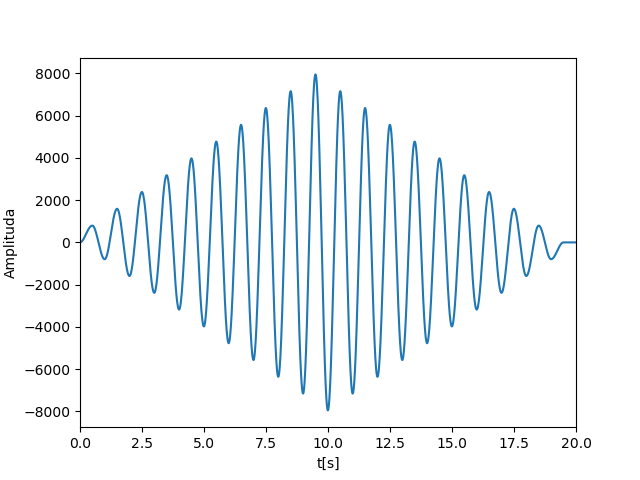
\includegraphics[scale=0.6]{splotSinusProstokat.png}
\caption{Operacja splotu funkcji sinusoidalnej i prostokątnej}
\end{figure}

\begin{figure}[H]
\centering
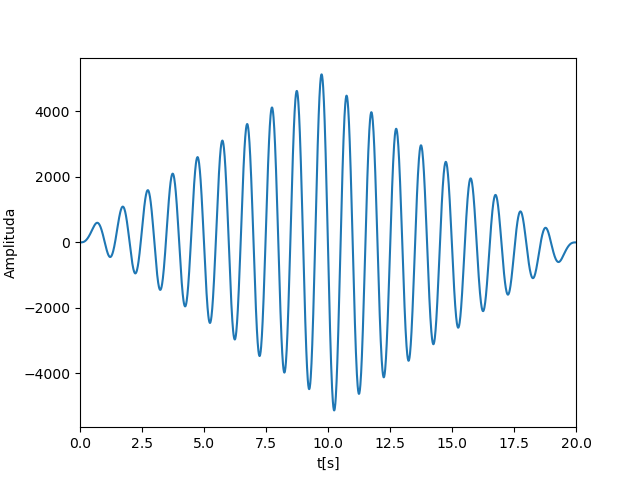
\includegraphics[scale=0.6]{splotTrojkatSinus.png}
\caption{Operacja splotu funkcji trójkątnej i sinusoidalnej}
\end{figure}

\subsection{Operacje korelacji}
\begin{figure}[H]
\centering
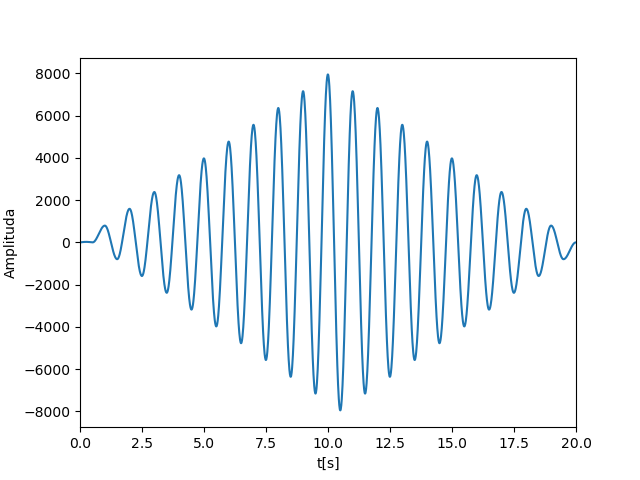
\includegraphics[scale=0.6]{korelacjaSinusProstokat.png}
\caption{Operacja korelacji bezpośredniej dla funkcji sinusoidalnej i prostokątnej}
\end{figure}

\begin{figure}[H]
\centering
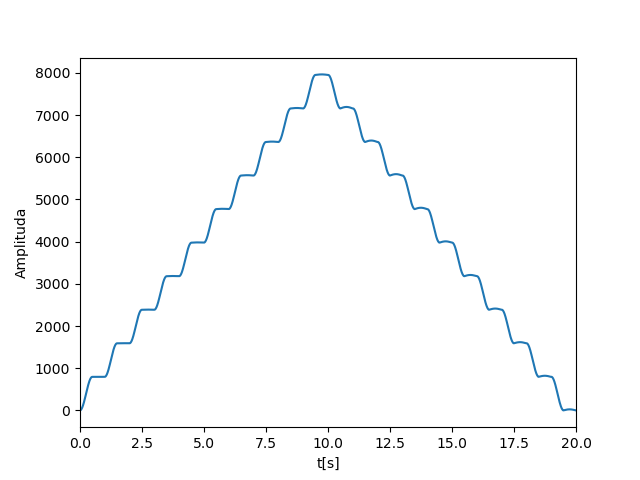
\includegraphics[scale=0.6]{korelacjaProstokatDwupolowkowy.png}
\caption{Operacja korelacji bezpośredniej dla funkcji prostokątnej i sinus. wyprostowanej dwupołówkowo}
\end{figure}

\begin{figure}[H]
\centering
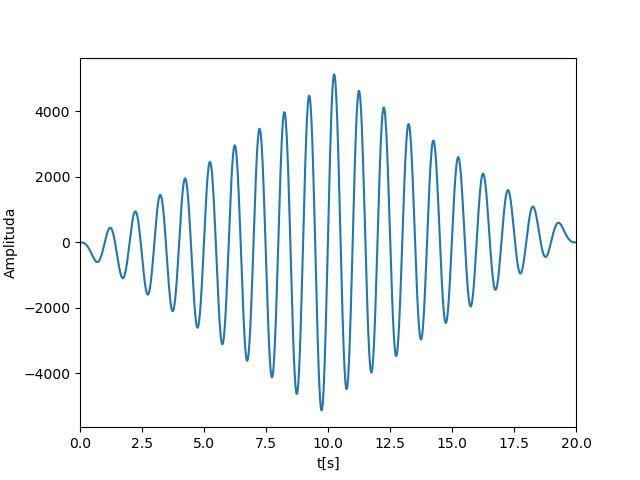
\includegraphics[scale=0.6]{korelacjaTrojkatSinus.png}
\caption{Operacja korelacji bezpośredniej dla funkcji sinusoidalnej i trójkątnej}
\end{figure}

\begin{figure}[H]
\centering
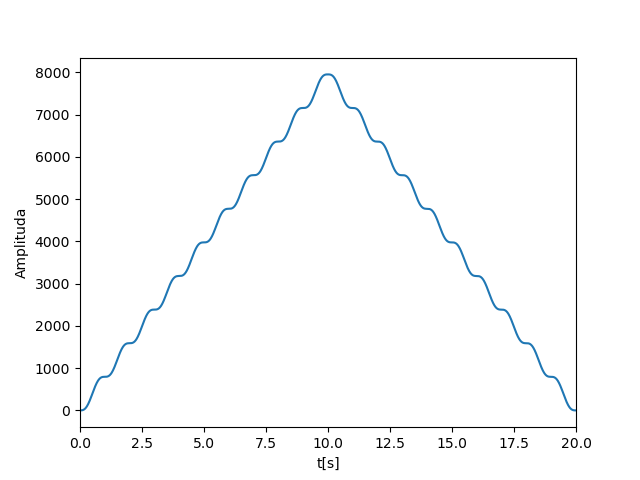
\includegraphics[scale=0.6]{korelacjaSplotTrojkatDwupolowkowy.png}
\caption{Operacja korelacji przez splot dla funkcji trójkątnej i sinus. wyprostowanej dwupołówkowo}
\end{figure}

\begin{figure}[H]
\centering
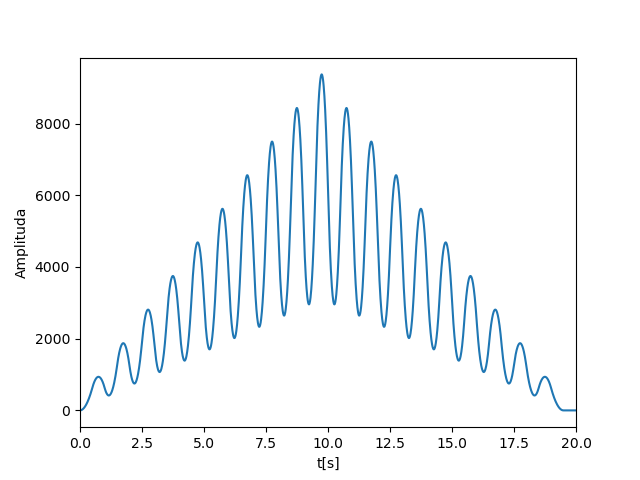
\includegraphics[scale=0.6]{korelacjaSplotTrojkatProstokat.png}
\caption{Operacja korelacji przez splot dla funkcji trójkątnej i prostokątnej}
\end{figure}

\subsection{Operacje filtracji z wykorzystaniem okna}
Celem eksperymentu jest przedstawienie wyników procesu filtracji sygnałów zaszumionych z i bez wykorzystania okna. O parametrach:
\begin{itemize}
\item amplituda: 5
\item okres: 3
\item czas początkowy: 0
\item czas trwania: 10
\end{itemize}

\begin{itemize}
\item Rząd filtru (M): 57
\item Częstotliwość odcięcia filtru (f0): 1
\item Częstotliwość próbkowania sygnału(fd): 250
\end{itemize}

\subsubsection{Rezultat}
\begin{figure}[H]
\centering
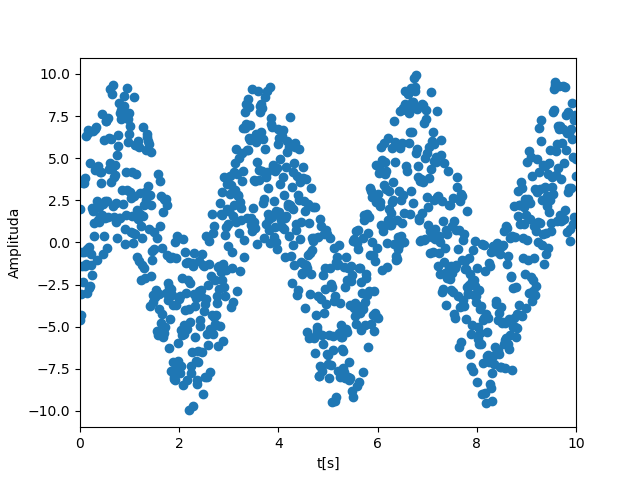
\includegraphics[scale=0.6]{sinusSzum.png}
\caption{Zaszumiony sygnał sinusoidalny}
\end{figure}

\begin{figure}[H]
\centering
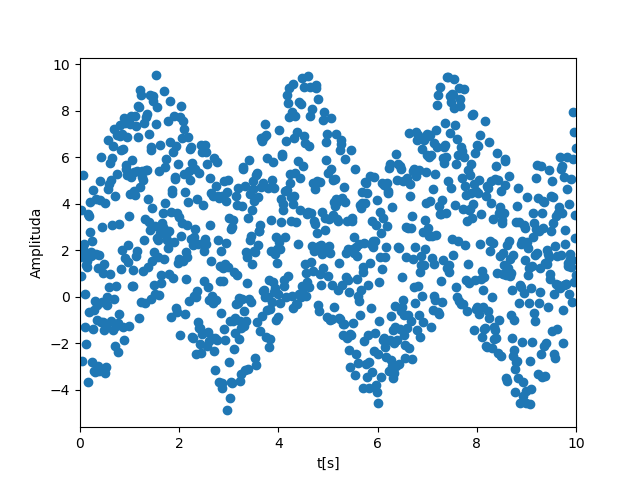
\includegraphics[scale=0.6]{trojkatSzum.png}
\caption{Zaszumiony sygnał trojkatny}
\end{figure}

\begin{figure}[H]
\centering
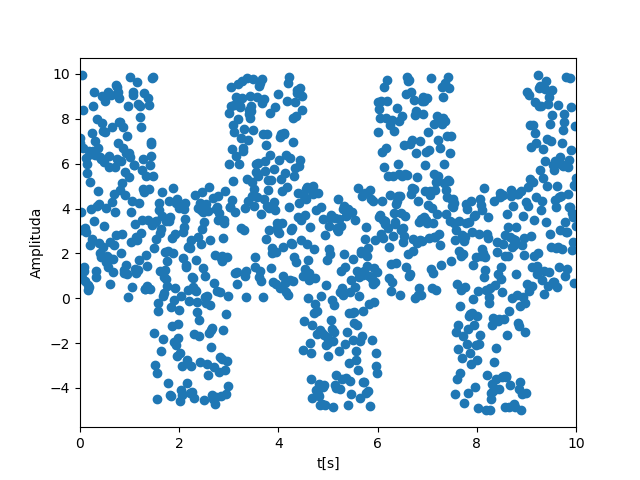
\includegraphics[scale=0.6]{prostokatSzum.png}
\caption{Zaszumiony sygnał prostokątny}
\end{figure}

\begin{figure}[H]
\centering
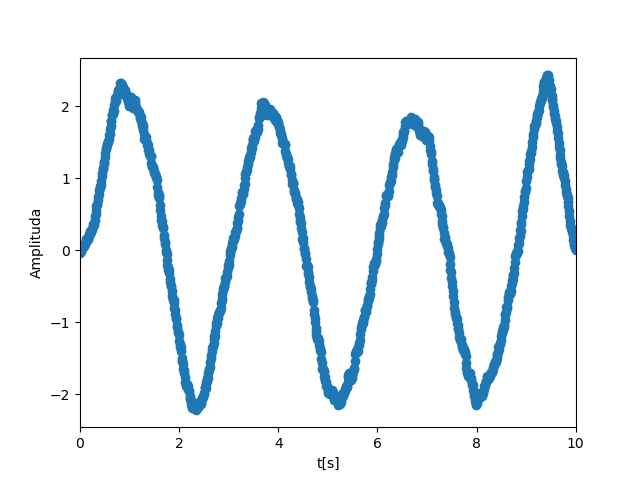
\includegraphics[scale=0.6]{filtrDolSinus.png}
\caption{Filtr dolnoprzepustowy dla funkcji sinusoidalnej}
\end{figure}

\begin{figure}[H]
\centering
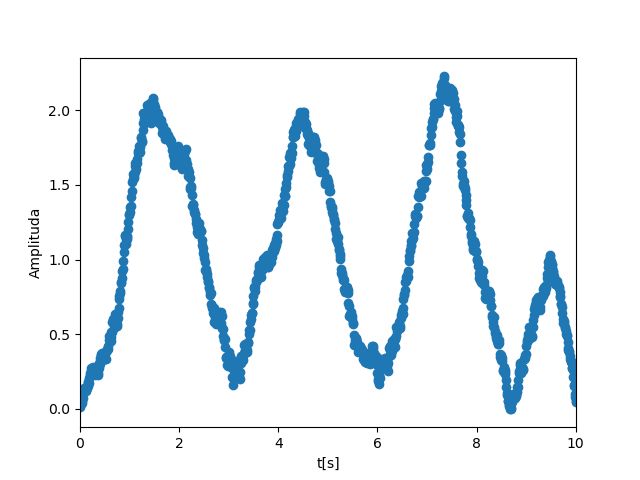
\includegraphics[scale=0.6]{filtrDolTrojkat.png}
\caption{Filtr dolnoprzepustowy dla funkcji trójkątnej}
\end{figure}

\begin{figure}[H]
\centering
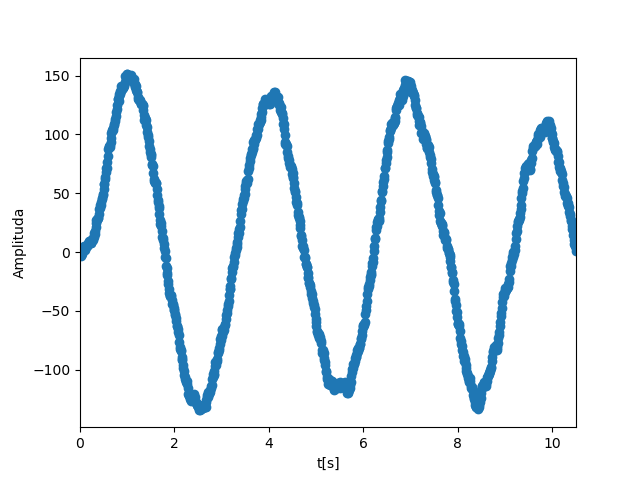
\includegraphics[scale=0.6]{filtrSrodekHanningSinus.png}
\caption{Filtr środkowoprzepustowy z oknem Hanninga dla funkcji sinusoidalnej}
\end{figure}

\begin{figure}[H]
\centering
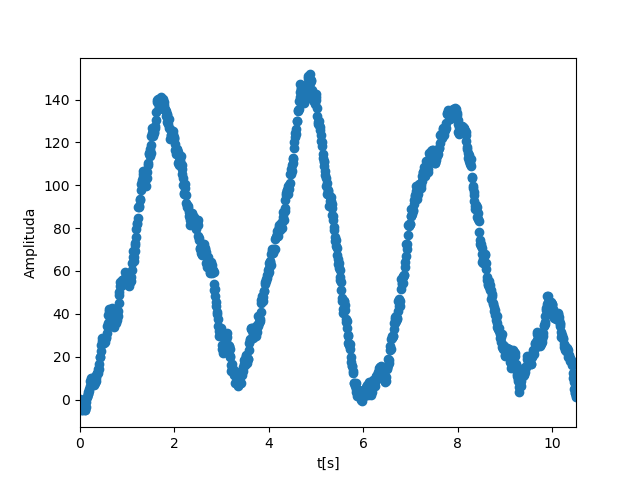
\includegraphics[scale=0.6]{filtrSrodekHanningTrojkat.png}
\caption{Filtr środkowoprzepustowy z oknem Hanninga dla funkcji trójkątnej}
\end{figure}

\begin{figure}[H]
\centering
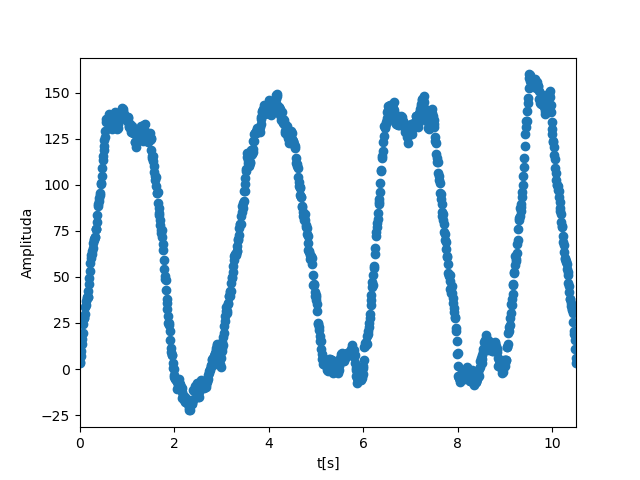
\includegraphics[scale=0.6]{filtrSrodekHanningProstokat.png}
\caption{Filtr środkowoprzepustowy z oknem Hanninga dla funkcji prostokątnej}
\end{figure}


\subsection{Antena - pomiar odległości}
Jednym ze sposobów wykorzystania otrzymanych rezultatów porównania sygnałów przesuniętych jest pomiar odległości od celu za pomocą radaru. Radar wysyła sygnał, który po odbiciu od obiektu powraca do anteny z opóźnieniem . Wykorzystując właśnie to opóźnienie i korelację sygnału wysłanego i zwrotnego. W poniższej tabeli przedstawiamy wyniki dla obliczonych odległości tj. odległość oryginalną, obliczony dystans oraz różnicę między nimi.
\\
\begin{itemize}
\item Liczba pomiarów: 10
\item Prędkość rzeczywista: 10
\item Prędkość w abstrakcyjnym ośrodku: 1000
\item Okres sygnału: 1
\item Częstotliwość próbkowania: 100
\item Długość buforów: 500
\end{itemize}

\begin{center}
 \begin{tabular}{||c c c c||} 
 \hline
 Oryginalny dystans & Obliczony dystans  \\ [0.5ex] 
 \hline\hline
 0 & 1.841  \\ 
 \hline
 10 & 8.123  \\
 \hline
 20 & 18.162 \\
 \hline
 30 & 28.111 \\
 \hline
 40 & 38.127 \\ 
 \hline
 50 &48.092  \\ 
 \hline
 60 & 58.131  \\
 \hline
 70 & 68.088  \\
 \hline
 80 & 78.096  \\
 \hline
 90 & 88.066  \\ 
 \hline
\end{tabular}
\end{center}


\section{Wnioski}
\begin {itemize}
\item Prezentowane wyniki są dowodem na poprawne wykonanie zadania tj. poprawność wykonania operacji splotu, korelacji bezpośredniej, korelacji z użyciem splotu, wykorzystaniu filtrów, oraz filtrów z oknami.
\end {itemize}


\begin{thebibliography}{0}
\bibitem{bib1}
\label{zad1}
\textit{Zadanie 2 - Próbkowanie i kwantyzacja} Cyfrowe Przetwarzanie Sygnału WIKAMP FTIMS\newline
\end{thebibliography}

\end{document}